\section{Diagrammi di sequenza} \label{seqDiag}

	\subsection{Diagramma di generazione metrica}

        \begin{figure}[htbp]
            \centering
            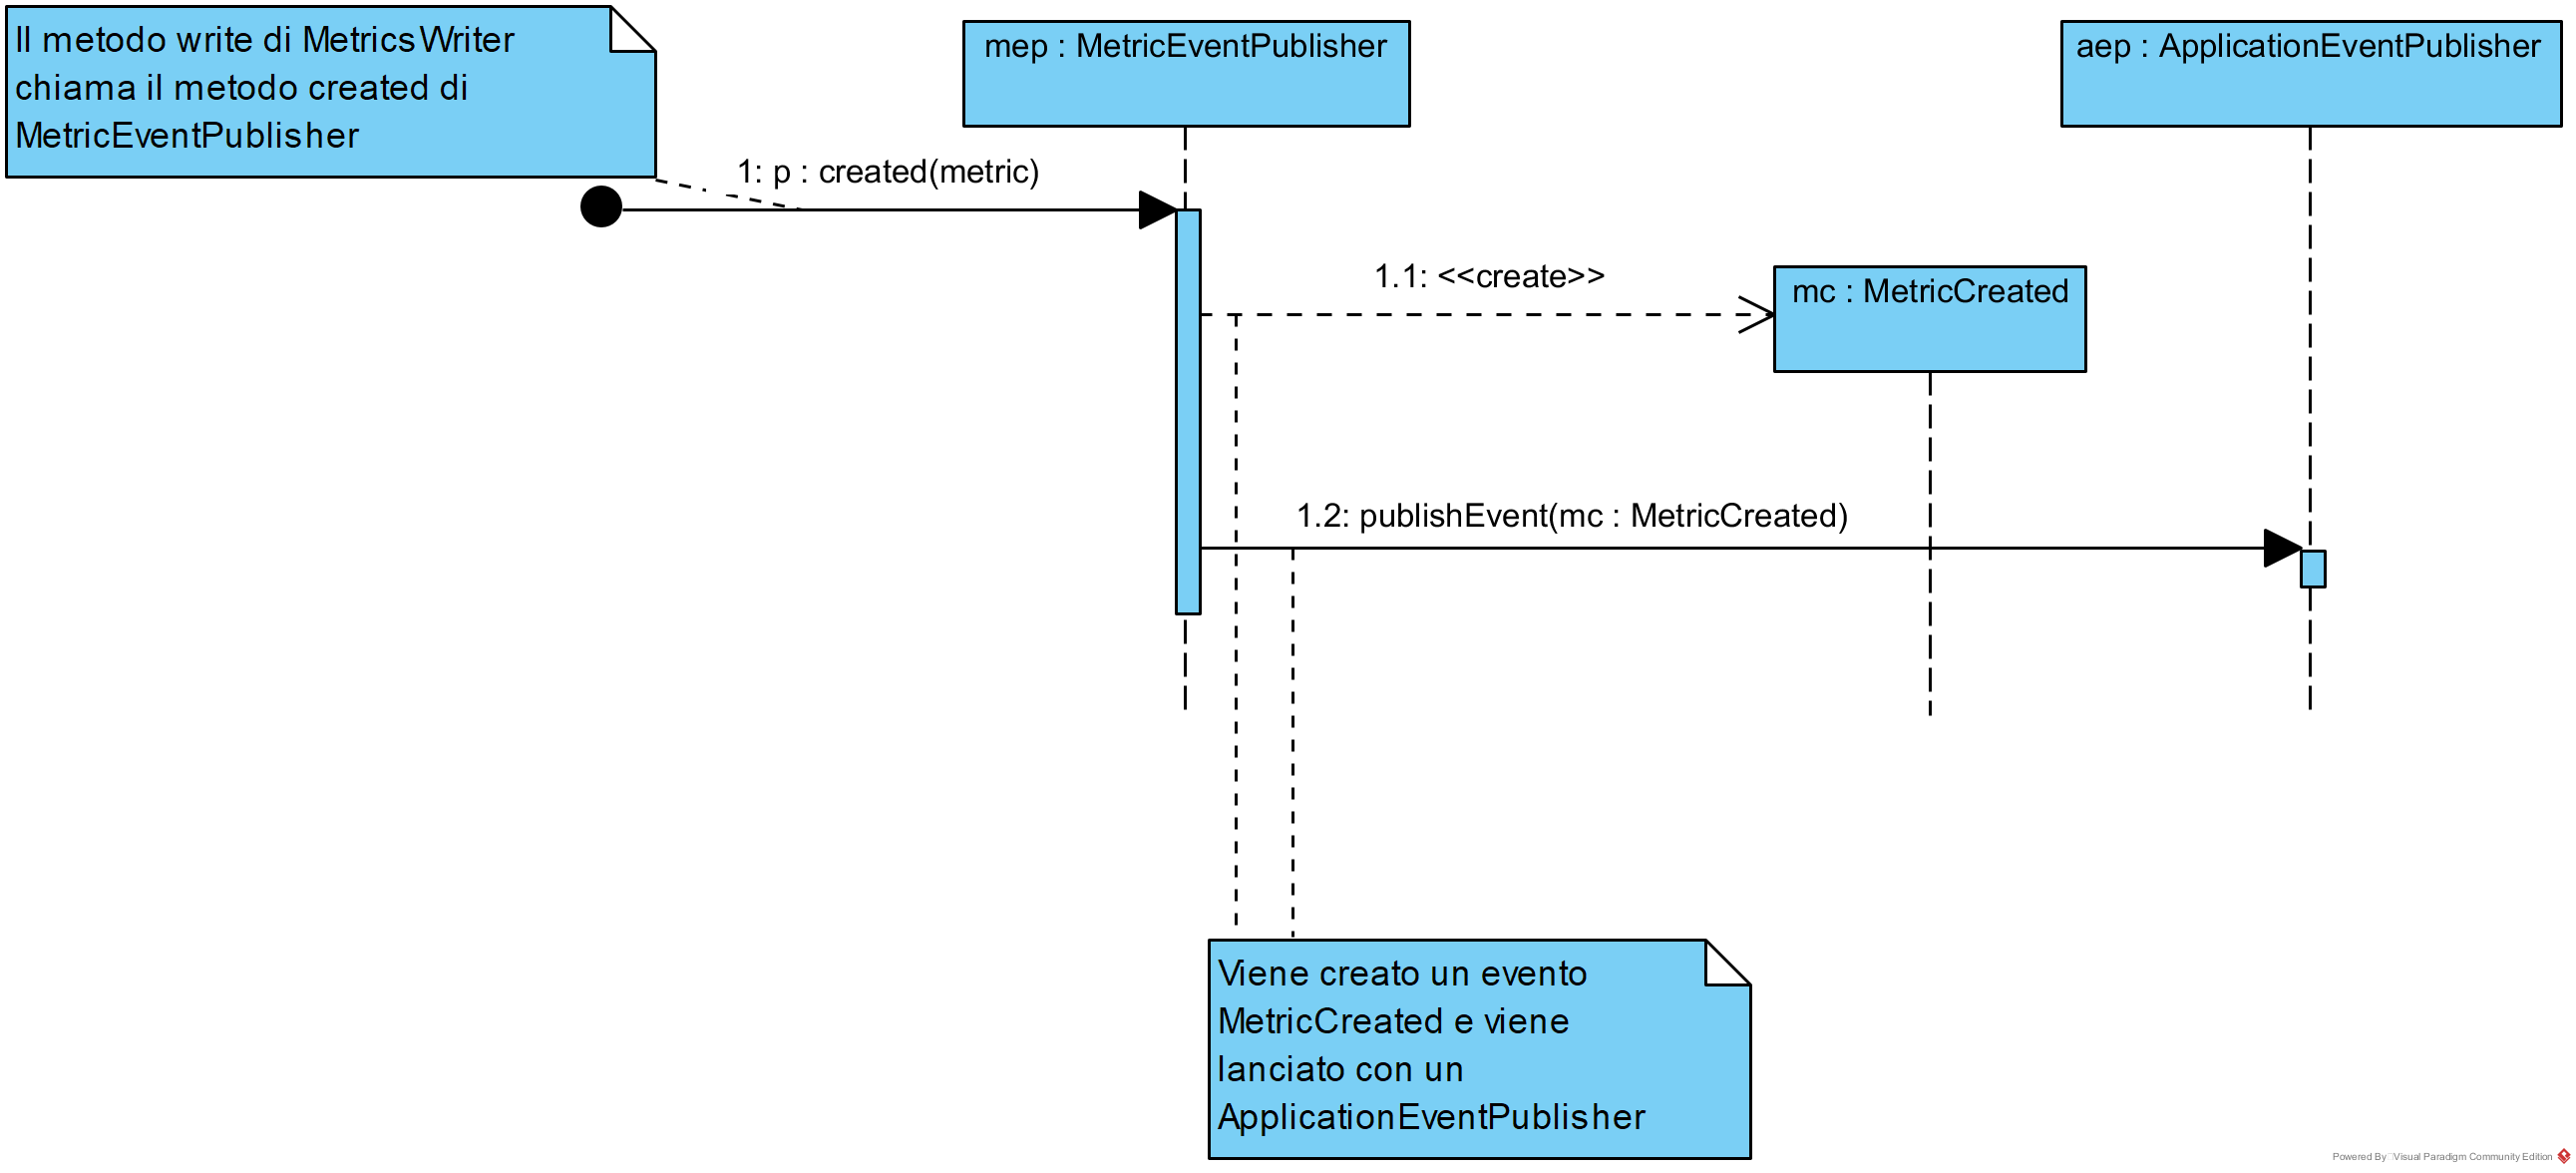
\includegraphics[width=\textwidth]{./img/DiagrammiSequenza/generatedMetricEvent.png}
            \caption[Diagramma di sequenza di generazione metrica]{Diagramma di sequenza che mostra le operazioni per generare una metrica}
        \end{figure}
        Il diagramma di sequenza mostra le operazioni per la generazione di una metrica. Il flusso è il seguente:
        \begin{enumerate}
        	\item viene notificato il MetricEventPublisher della creazione di una metrica tramite il metodo created;
        	\item MetricEventPublisher si occupa di creare un evento MetricCreated e di lanciarlo tramite un'ApplicationEventPublisher.
        \end{enumerate}
        
    \newpage
    
    \subsection{Diagramma MetricCreated - AlertsManager}

        \begin{figure}[htbp]
            \centering
            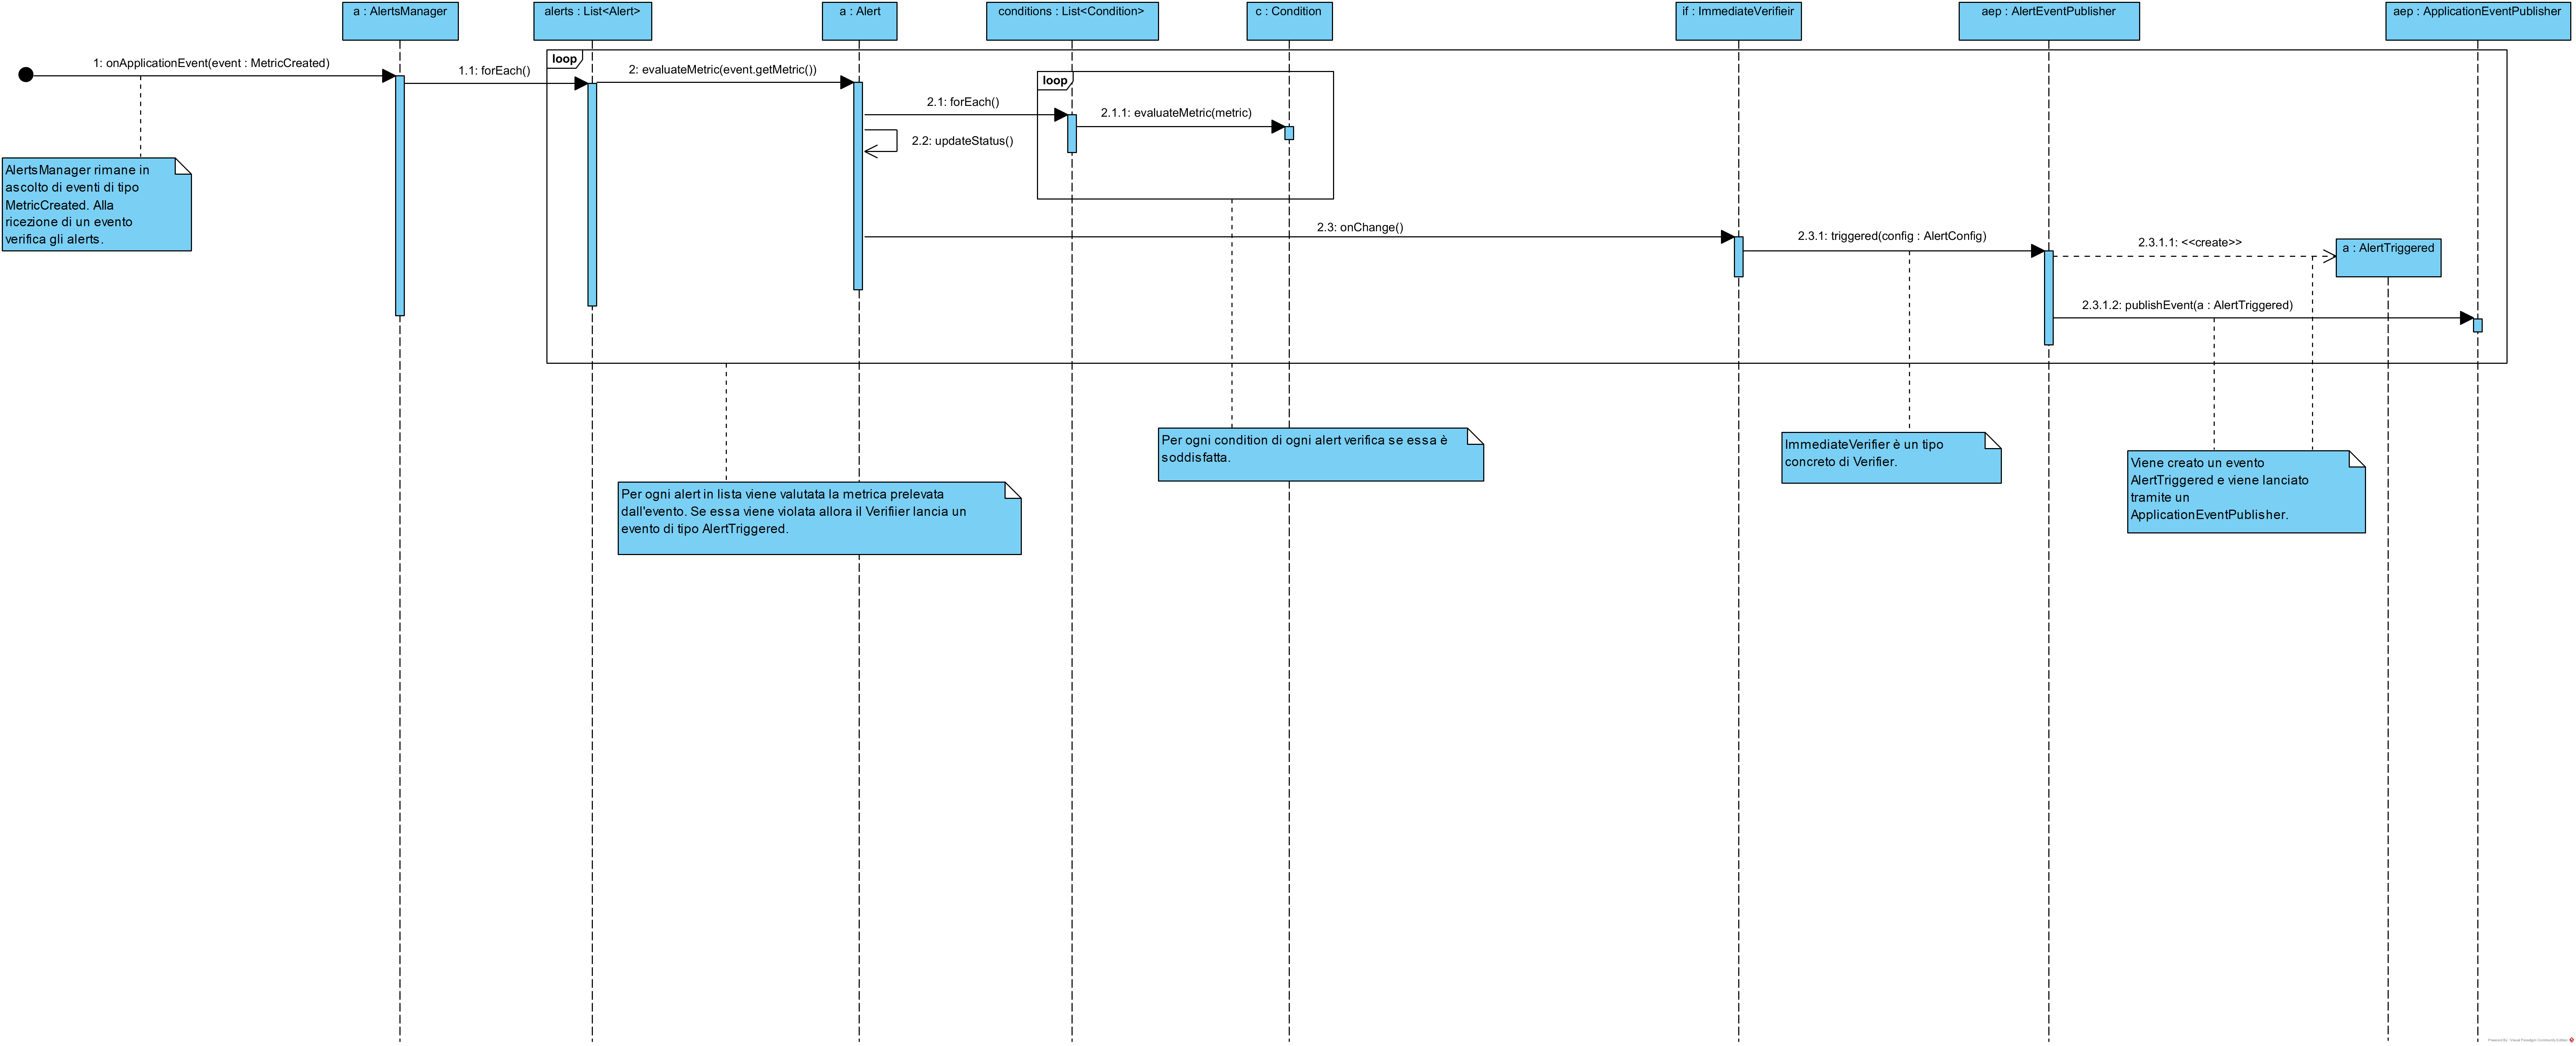
\includegraphics[width=\textwidth]{./img/DiagrammiSequenza/alertsManager.png}
            \caption[Diagramma di sequenza MetricCreated - AlertsManager]{Diagramma di sequenza delle operazioni di AlertsManager}
        \end{figure}
        Il diagramma di sequenza rappresenta le operazioni della classe AlertsManager. Il flusso è il seguente:
        \begin{enumerate}
        	\item AlertsManager rimane in ascolto di un evento MetricCreated;
        	\item per ogni alert in lista viene valutata la metrica prelevata dall'evento;
        	\item la valutazione avviene tramite valutazione di tutte le conditions di ogni alert;
        	\item in caso di criticità un verificatore invocherà il metodo triggered dell'AlertEventPublisher;
        	\item AlertEventPublisher si occupa di creare un evento AlertTriggered e di lanciarlo con un ApllicationEventPublisher.
        \end{enumerate}
        
    \newpage

    \subsection{Diagramma AlertTriggered - ActionsManager}

        \begin{figure}[htbp]
            \centering
            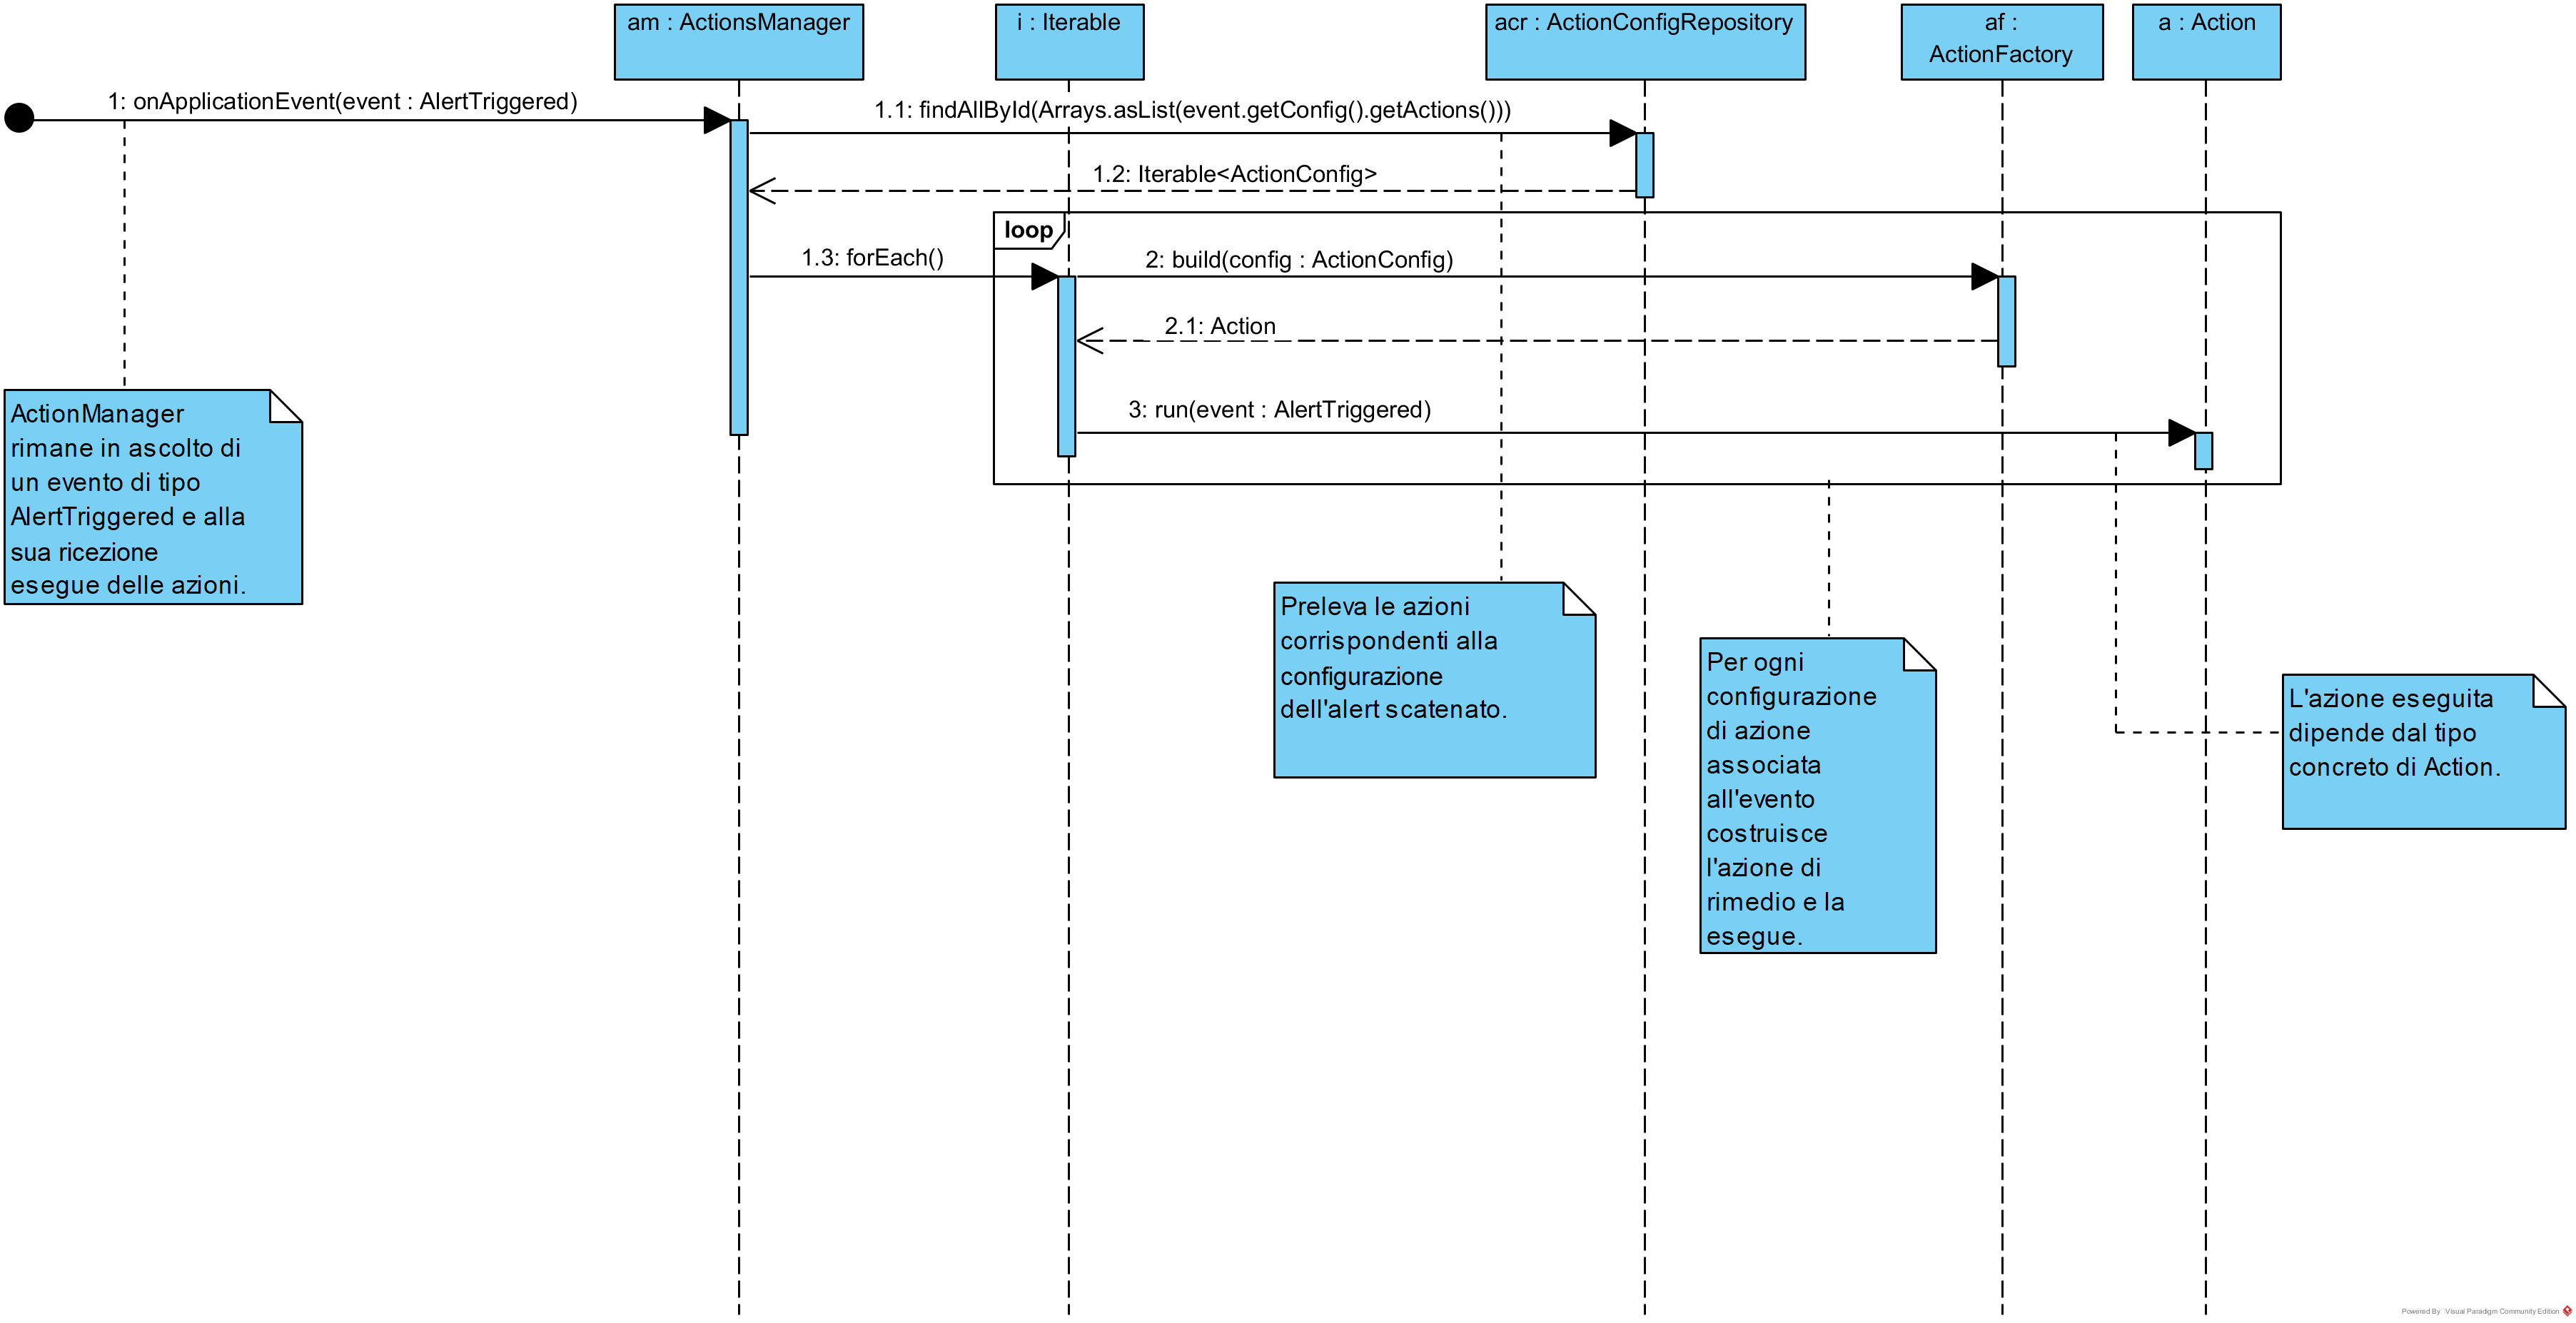
\includegraphics[width=\textwidth]{./img/DiagrammiSequenza/ActionsManager.png}
            \caption[Diagramma di sequenza AlertTriggered - ActionsManager]{Diagramma di sequenza delle operazioni di ActionsManager}
        \end{figure}
        Il diagramma di sequenza rappresenta le operazioni della classe ActionsManager. Il flusso è il seguente:
        \begin{enumerate}
        	\item ActionsManager rimane in ascolto di un evento AlertTriggered;
        	\item alla ricezione dell'evento vengono raccolte dal database le configurazioni delle azioni associate all'evento;
        	\item per ogni configurazione di azione, essa viene costruita tramite factory pattern e successivamente eseguita.
        \end{enumerate}

\newpage

    
